\chapter{Development components}
\label{ch:development-components}

\section{Development workflow}
\label{sec:development-workflow}

\begin{figure}
\centering
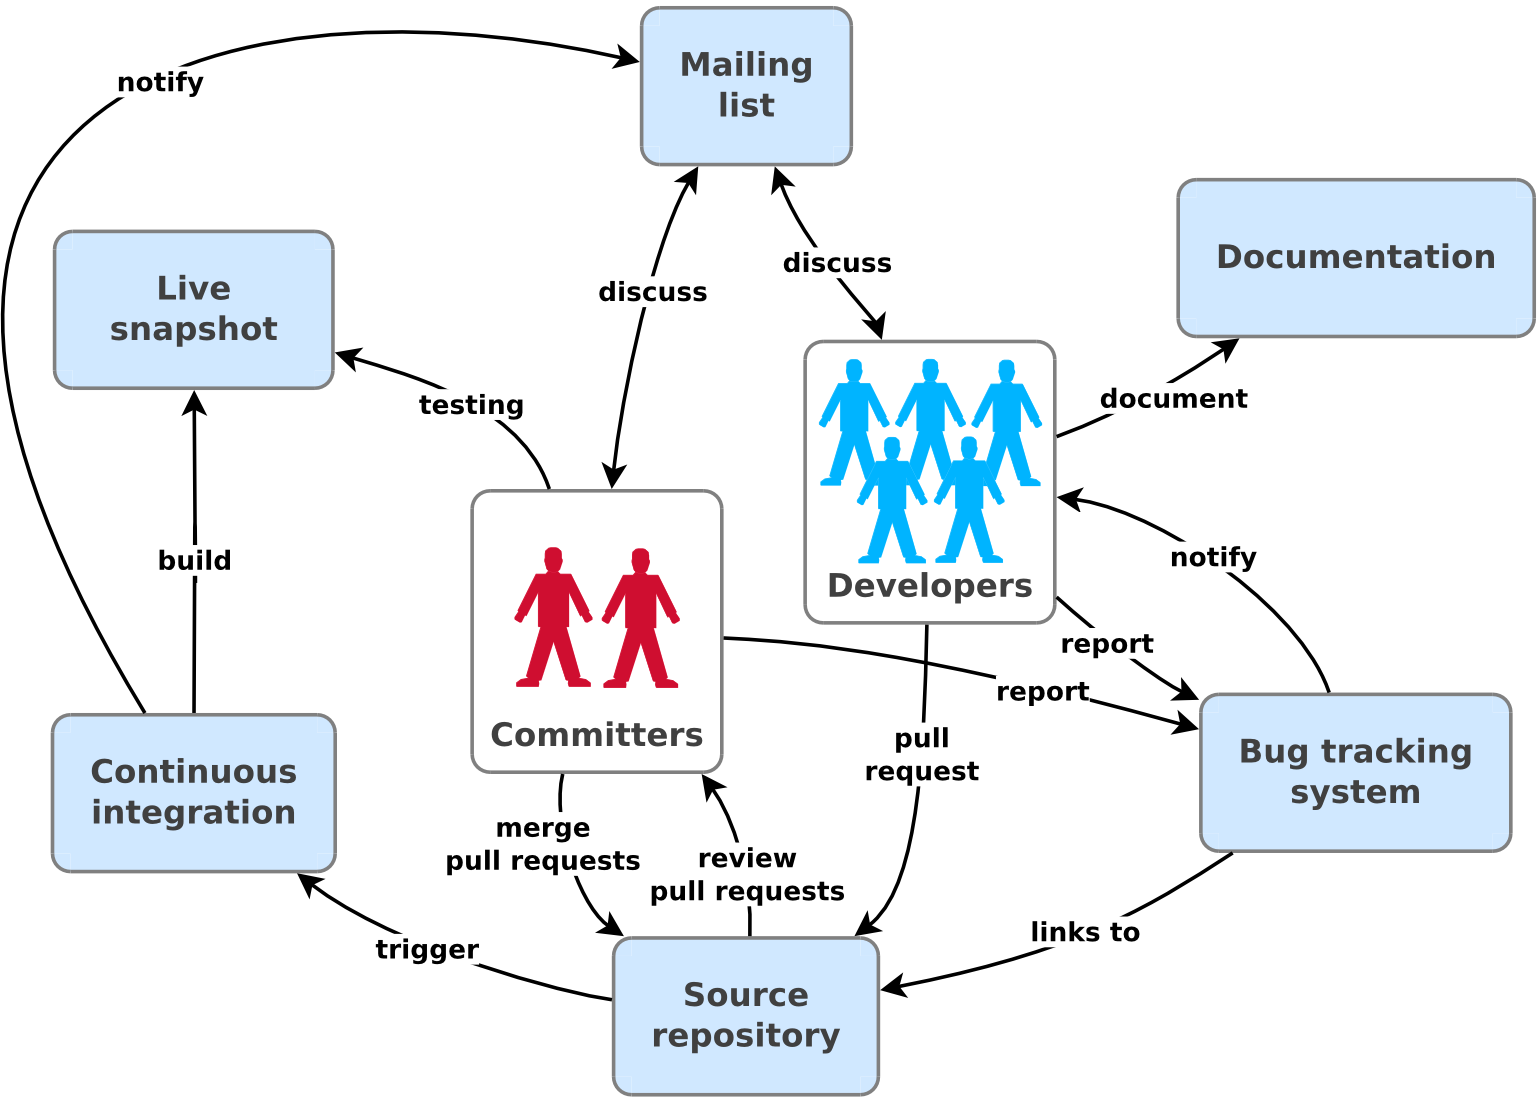
\includegraphics[width=0.67\textwidth]{images/development-workflow.png}
\caption{Development workflow with all tools}
\label{fig:development-workflow}
\end{figure}

\section{Details}
\label{sec:details}

The Figure~\ref{fig:development-workflow} illustrates the global development workflow.
In this workflow, there will be developers and integrators who interact using a variety of tools.
We will now give more details on these tools and how they will be used.

\subsection{Mailing list}
\label{sec:mailing-list}

An email mailing list will be available for general decision making about the platform,
the goal being to keep records of discussions and choices about developments or architecture design.

\subsection{Source repository}
\label{sec:source-repository}

A distributed source code repository will be provided for storing the source code or binaries
needed for building the \learnpad platform. The main repository will be stored in a public GitHub,
repository. Github is a popular code hosting and collaborative software development environment
which is free to non-private projects. Github provides not only a place to store the code but also
a rich variety of tools such as issue tracking, ability to browse code and readme files in a web
browser, advanced email notification, and well documented applications for all popular computer
Operating Systems.

Each developers will work on his own copy (or \emph{fork}) of the repository and propose new
functionality or bug fixes using Github \emph{pull requests}\footnote{A pull request is a method of
submitting contributions to a software project. It contains the \emph{patch} representing changes to
be made and creates a central place for those changes to be reviewed and discussed} which
integrators will have the duty to review. An integrator may accept the \emph{pull request},
request changes or further information or in an extreme case, close it pending further discussion.

Despite having direct access to the shared repository, an integrator who is also a developer should
make sure to use \emph{pull requests} for integrating their own functionality so as to allow for
discussion with other integrators and developers and to keep record of the contribution.

All developers should adopt the \emph{check in early and often} development methodology.
Code in development is not expected to be bug-free but great importance is placed on collaboration
and working in the open. In a fast-changing collaborative software development project, frequent
pull requests help everybody. They help the developer making them because he is able to avoid
rewriting code to cope with changes in other elements of the system and they also help other
developers who are able to see and adapt to changes in this developer's component.

\subsection{Documentation}
\label{sec:documentation}

An XWiki instance has already been provided and is currently being used for collaboration and
documentation. Documentation will be able to be written accompanying the source code in the
repository or it may be placed on the wiki as long as relevant documents are referenced from the
source repository. The main entry point into the documentation for each partner's sub-folder will
be a file called \texttt{readme.md} (see Section~\ref{sec:source-structure} for more information
about partner sub-folders.)

\subsection{Bug tracking system}
\label{sec:bug tracking-system}

All participants will be responsible for the discovery and diagnosis of bugs. Bugs, feature
requests, \emph{pull requests} and other to-do items shall be submitted to the Github bug tracking
system where others can keep track of issues which need to be addressed. Email notifications of new
issues will be sent to integrators and updates of an issue will be sent to those who participate in
(EG: comment on) the issue.

\subsection{Continuous Integration Server}
\label{sec:ci-server}

Continuous integration will be provided by travis-ci, a hosted, distributed continuous integration
service used to build and test projects hosted at GitHub. Like Github, travis-ci service is free
for public projects and travis-ci provides email notification of build failures and GitHub
integration for automatically testing \emph{pull requests} before they are merged.
The Operating System on travis-ci build machines is Ubuntu Linux 12.04 LTS\footnote{The stable
version of a widely used Linux distribution.} which will heretofore be referred to as the
\emph{target system}, all parts of the online platform will be expected to build and run on this
system. Travis-ci is also capable of uploading and downloading files from other servers as part of
the build and of storing secret keys which may be used to encrypt parts of a configuration which
are considered sensitive.
